\begin{frame}{Coupled System for Rectilinear Flow}
	\scriptsize
We consider $\boldsymbol{u} = \left( 0, 0, w(x,y, t)\right)^T$, $f(x,y,t,\phi,\theta)$. We get
\begin{equation}
	\begin{aligned}
		&\sin\theta \partial_{t}f(x,y,t,\phi, \theta)+ \textcolor{red}{\partial_x(\cos\phi \sin\theta \cos\theta f)} + \textcolor{red}{\partial_y(\sin \phi \sin \theta \cos \theta f)} \\
		&+ \textcolor{blue}{\partial_\theta\left(( w_x \sin^3 \theta \cos \phi + w_y\sin \phi \sin^3 \theta) f\right)}
		= \textcolor{blue}{D_{r}\left( \partial_\phi \left(\frac{1}{\sin \theta} \partial_\phi f \right)+ \partial_\theta (\sin \theta \partial_\theta f)\right)} \\
		&Re\partial_{t}w(x,y,t) = \partial_{xx}w + \partial_{yy}w + \delta\left(\bar{\rho}-\int_{0}^{2\pi} \int_{0}^{\pi} f \sin \theta d\theta d\phi \right).
	\end{aligned}
\end{equation}
The system of hierarchy of moment equations is given as
	\begin{equation}
		\partial_t Q + \textcolor{red}{A  \partial_x Q}
		+ \textcolor{red}{B \partial_y Q} =  \textcolor{blue}{ D(w_x,w_y)Q+ D_rEQ}.
	\end{equation}
\end{frame}

\begin{frame}
	\scriptsize
	\begin{figure}[H]
	\centering
	\begin{minipage}{0.4\textwidth}
		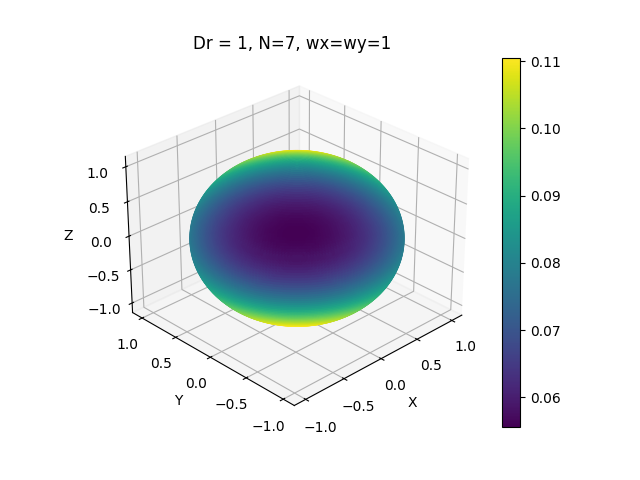
\includegraphics[scale=0.28]{Bilder_wxwy/Sol_onSphere_wx=1=wy_Dr=1_N=7}
	\end{minipage}
	\hfill 
	\begin{minipage}{0.4\textwidth}
		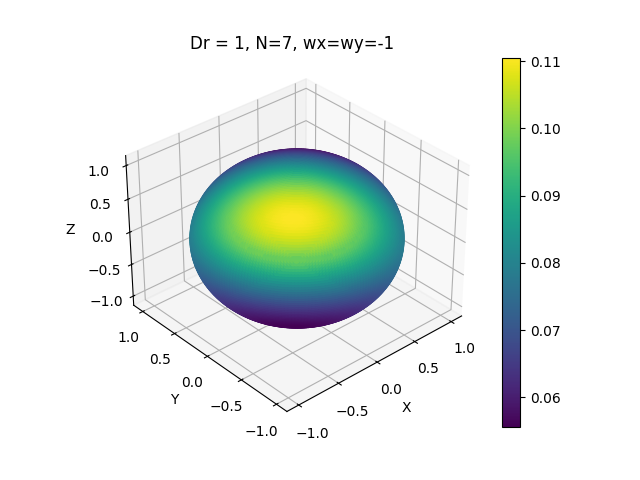
\includegraphics[scale=0.28]{Bilder_wxwy/Sol_onSphere_wx=-1=wy_Dr=1_N=7}
	\end{minipage}
   \caption{Numerical solution of the drift-diffusion term for fixed $w_x$ and $w_y$.}
	\begin{minipage}{0.4\textwidth}
		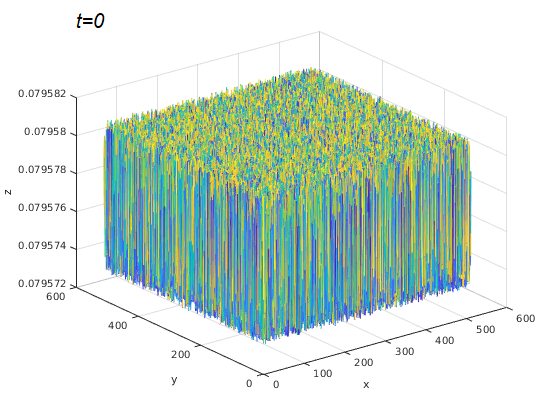
\includegraphics[scale=0.25]{Bilder_wxwy/4th_t=0_mx=my=512_random}
	\end{minipage}
	\hfill 
	\begin{minipage}{0.4\textwidth}
	    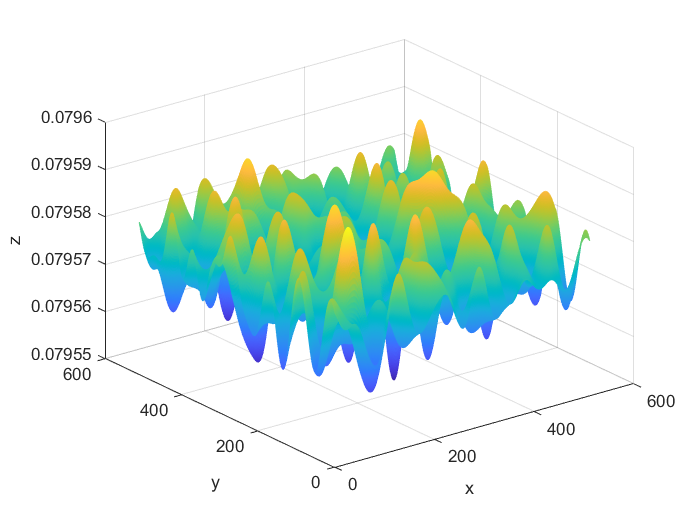
\includegraphics[scale=0.25]{Bilder_wxwy/4th_t=100_mx=my=512_random}
    \end{minipage}
 \caption{Solution structure of $c^0_0$ with $N = 2$.}
    \end{figure}
\end{frame}

